\section{Introduction}

\subsection*{Terminology}
\begin{frame}
\frametitle{Springy Leg Offset Mass}
\begin{columns}
\column{0.5\textwidth}
\begin{figure}
\centering
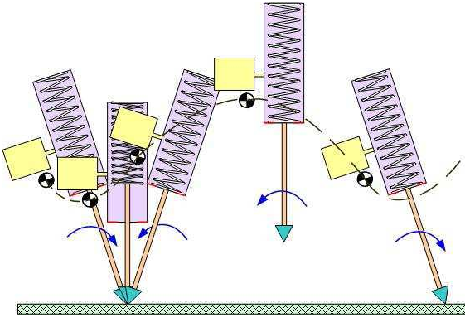
\includegraphics[width=\textwidth]{fig/SLOM_motion.pdf}
\caption{SLOM motion}
\end{figure}

\column{0.5\textwidth}
\begin{block}{Stages}
\begin{itemize}
\item
Lift-off\\[0.1in]
\item
Free fall\\[0.1in]
\item
Touch-down\\[0.1in]
\item
Stance
\end{itemize}
\end{block}
\begin{block}{Terms}
\begin{itemize}
\item
Energy Pumping Mechanism\\[0.1in]
\item
Constraint\\[0.1in]
\item
Energy Release\\[0.1in]
\end{itemize}
\end{block}

\end{columns}
\end{frame}

\section[SLOM]{SLOM}
\subsection*{Previous Design}
\begin{frame}
\frametitle{Previous Work}
\begin{columns}

\uncover<1->{
\column{0.5\textwidth}
\begin{figure}
\centering
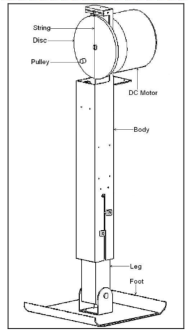
\includegraphics[width=0.5\textwidth]{fig/saboo.pdf}
\end{figure}

\tiny{
\begin{block}{SLOM hopper}
\begin{itemize}
\item
Compression spring
\item
Ratchet and paul activated by voice coil
\item
Large leg mass : Small hopping height
\item
In-place hopping : Feed forward control law
\end{itemize}
\end{block}
}
}

\uncover<2->{
\column{0.5\textwidth}
\begin{figure}
\centering
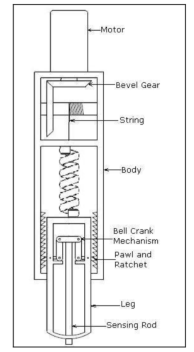
\includegraphics[width=0.4\textwidth]{fig/londhe.pdf}
\end{figure}

\vspace{0.2in}
\tiny{
\begin{block}{1D hopper}
\begin{itemize}
\item
Spring compressed by a motor
\item
Bell-crank constraint mechanism
\item
Use of impact to release energy
\end{itemize}
\end{block}
}
}
\end{columns}
\end{frame}



